%=============================================================================
\section{Design}

%-----------------------------------------------------------------------------
\subsection{Approach}

\enote{Explain data flow; calling approach based on passing buffers; in-process or cross-process. Explain using FlatBuffers and why. Explain in general terms that we deal directly with variables in a global space, with lightweight coordination to allocate variables; and why (avoid duplication/rewriting etc.}

zkInterface is a procedural, purely functional interface for zero-knowledge systems that enables cross-language interoperability via dynamic linking and shared memory. The current version, even if limiting, creates an interface based on R1CS formatting and offers the ability to abstractly craft a constraint system building from different components, possibly written in different frameworks, by determining how data should be written and read. 

\enote{I'm not sure what this means:}
It can also be seen as a design tool for improved generation of constraints and usability, analogous to a portable binary format, since one can parametrize the functions calls and easily compose different functions, or components, that are not directly compatible.

\begin{figure}[h!]
	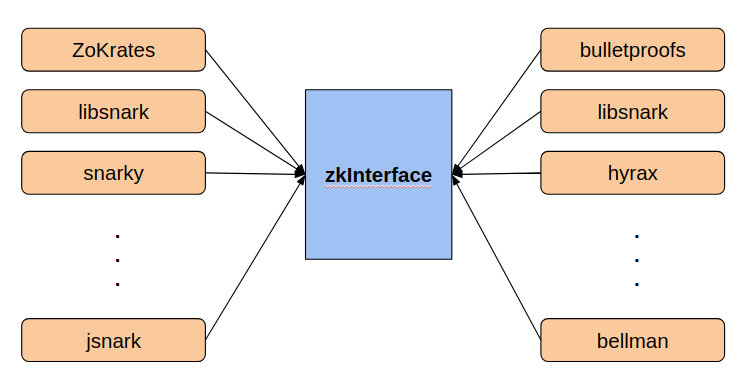
\includegraphics[width=\linewidth]{interface.png}
	\caption{zkInterface\enote{Replace by diagram on slack}}
	\label{interface}
\end{figure}



%-----------------------------------------------------------------------------
\subsection{Architecture}

\enote{Describe the high-level design, introducing all the main concepts in a readable narrative and referring to them concretely by the  identifier name in the sourcecode.}
		
		
\paragraph{Main functionality.}

The interface works across every zero-knowledge front-end and back-end, minimizing, when possible, the overhead of using a general format. This is achieved in several ways:

\begin{itemize}
	\item By using a protoboard-like method for shared memory allocation, and thus preventing double-copying the data unnecessarily.
	\item By parametrizing the function calls to the different components so to take advantage of the specific context underlying those components.
	\item By using FlatBuffers, an efficient cross platform serialization library for different languages. This tool allows us to easily write ad-hoc parsers from scratch and has a very low overhead in shared memory, which can be used in regular function calls. 
\end{itemize}


The two main purposes of the interface are the computations of the \emph{instance reduction}, which generates a portable circuit or constraint system, and the \emph{witness reduction}, which assigns values to the variables allocated in the instance reduction. We have designed the interface so that each of these two processes actually use the same exact routine, except with different message types.

Essentially, as seen in Figure \ref{flow}, the caller of the interface can be both an application or a component that requires a sub-component, an abstraction that helps make the interface minimal. Say I want to compute a proof of set membership by using a Merkle Tree of hashes. Then, the flow is the following:
\begin{enumerate} 
	\item The application will call the Merkle Tree component that exists in some front-end framework, which starts allocating in memory the variables and constraints in the standard R1CS format.
	\item For every hash computation needed to generate the path, the Merkle Tree will itself call a hasher sub-component, possibly from a different framework, by passing it the parameters, including the next free memory slot for allocating the hash constraints and variables.
	\item The hash component will then allocate in memory the constraints and variables, to which the Merkle Tree component is oblivious (except the shared input / outputs: the input message and the output hash digest).
	\item Specifically, for each call to the hash component, the input message is given as part of the request and the hash component sends the hash digest as part of the response. The rest of the variables are locally dealt with by the hash component but are shared in memory by all the components.
\end{enumerate}

Note how the routine can be re-used by the witness reduction and deterministically assign the values to the respective variables in memory. Moreover, if needed, the constraint system can be outputed as a file containing a static rank-1 constraint system. One objection to using this routine design is that the component at the top level (i.e.: the Merkle Tree) cannot is waiting for the response of the sub-component (i.e.: the hasher component). This can have a cost in the efficiency of the circuit generation if we imagine a long enough chain of sub-calls that would cause a quadratic overhead. This is unlikely to happen in the current set of applications and circuits. 
	
\begin{figure}[h!]
	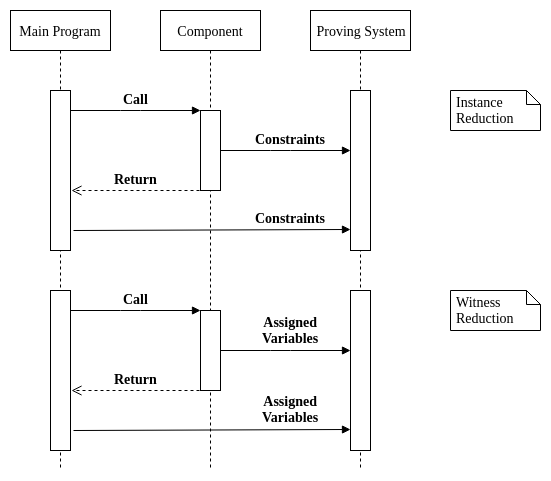
\includegraphics[width=\linewidth]{call_flow.png}
	\caption{The flow of messages between libraries using the interface}
	\label{flow}
\end{figure}

\subsection{Calling convention and file format}

\enote{Explain how these are mostly implied by FlatBuffers. Give any additional information necessary beyond that.}


\subsection{using zkInterface}

\enote{Explain, in concrete terms, what people need to do to use this standard. As a backend author? As a frontend framework author? As a guy who writes gadgets? As an integrator needing to bundle the dependencies?}
